\section{Software}

\subsection{Finite-Elemente-Methode (FEM)}
Zur Diskretisierung des Poisson-Problems, das betrachtet wird, kann man mit der implementierten FEM ein LGS $A u = b$ aufstellen, welches zur näherungsweisen Berechnung der Lösung dient. \\

\begin{figure}[h]
	\begin{center}
		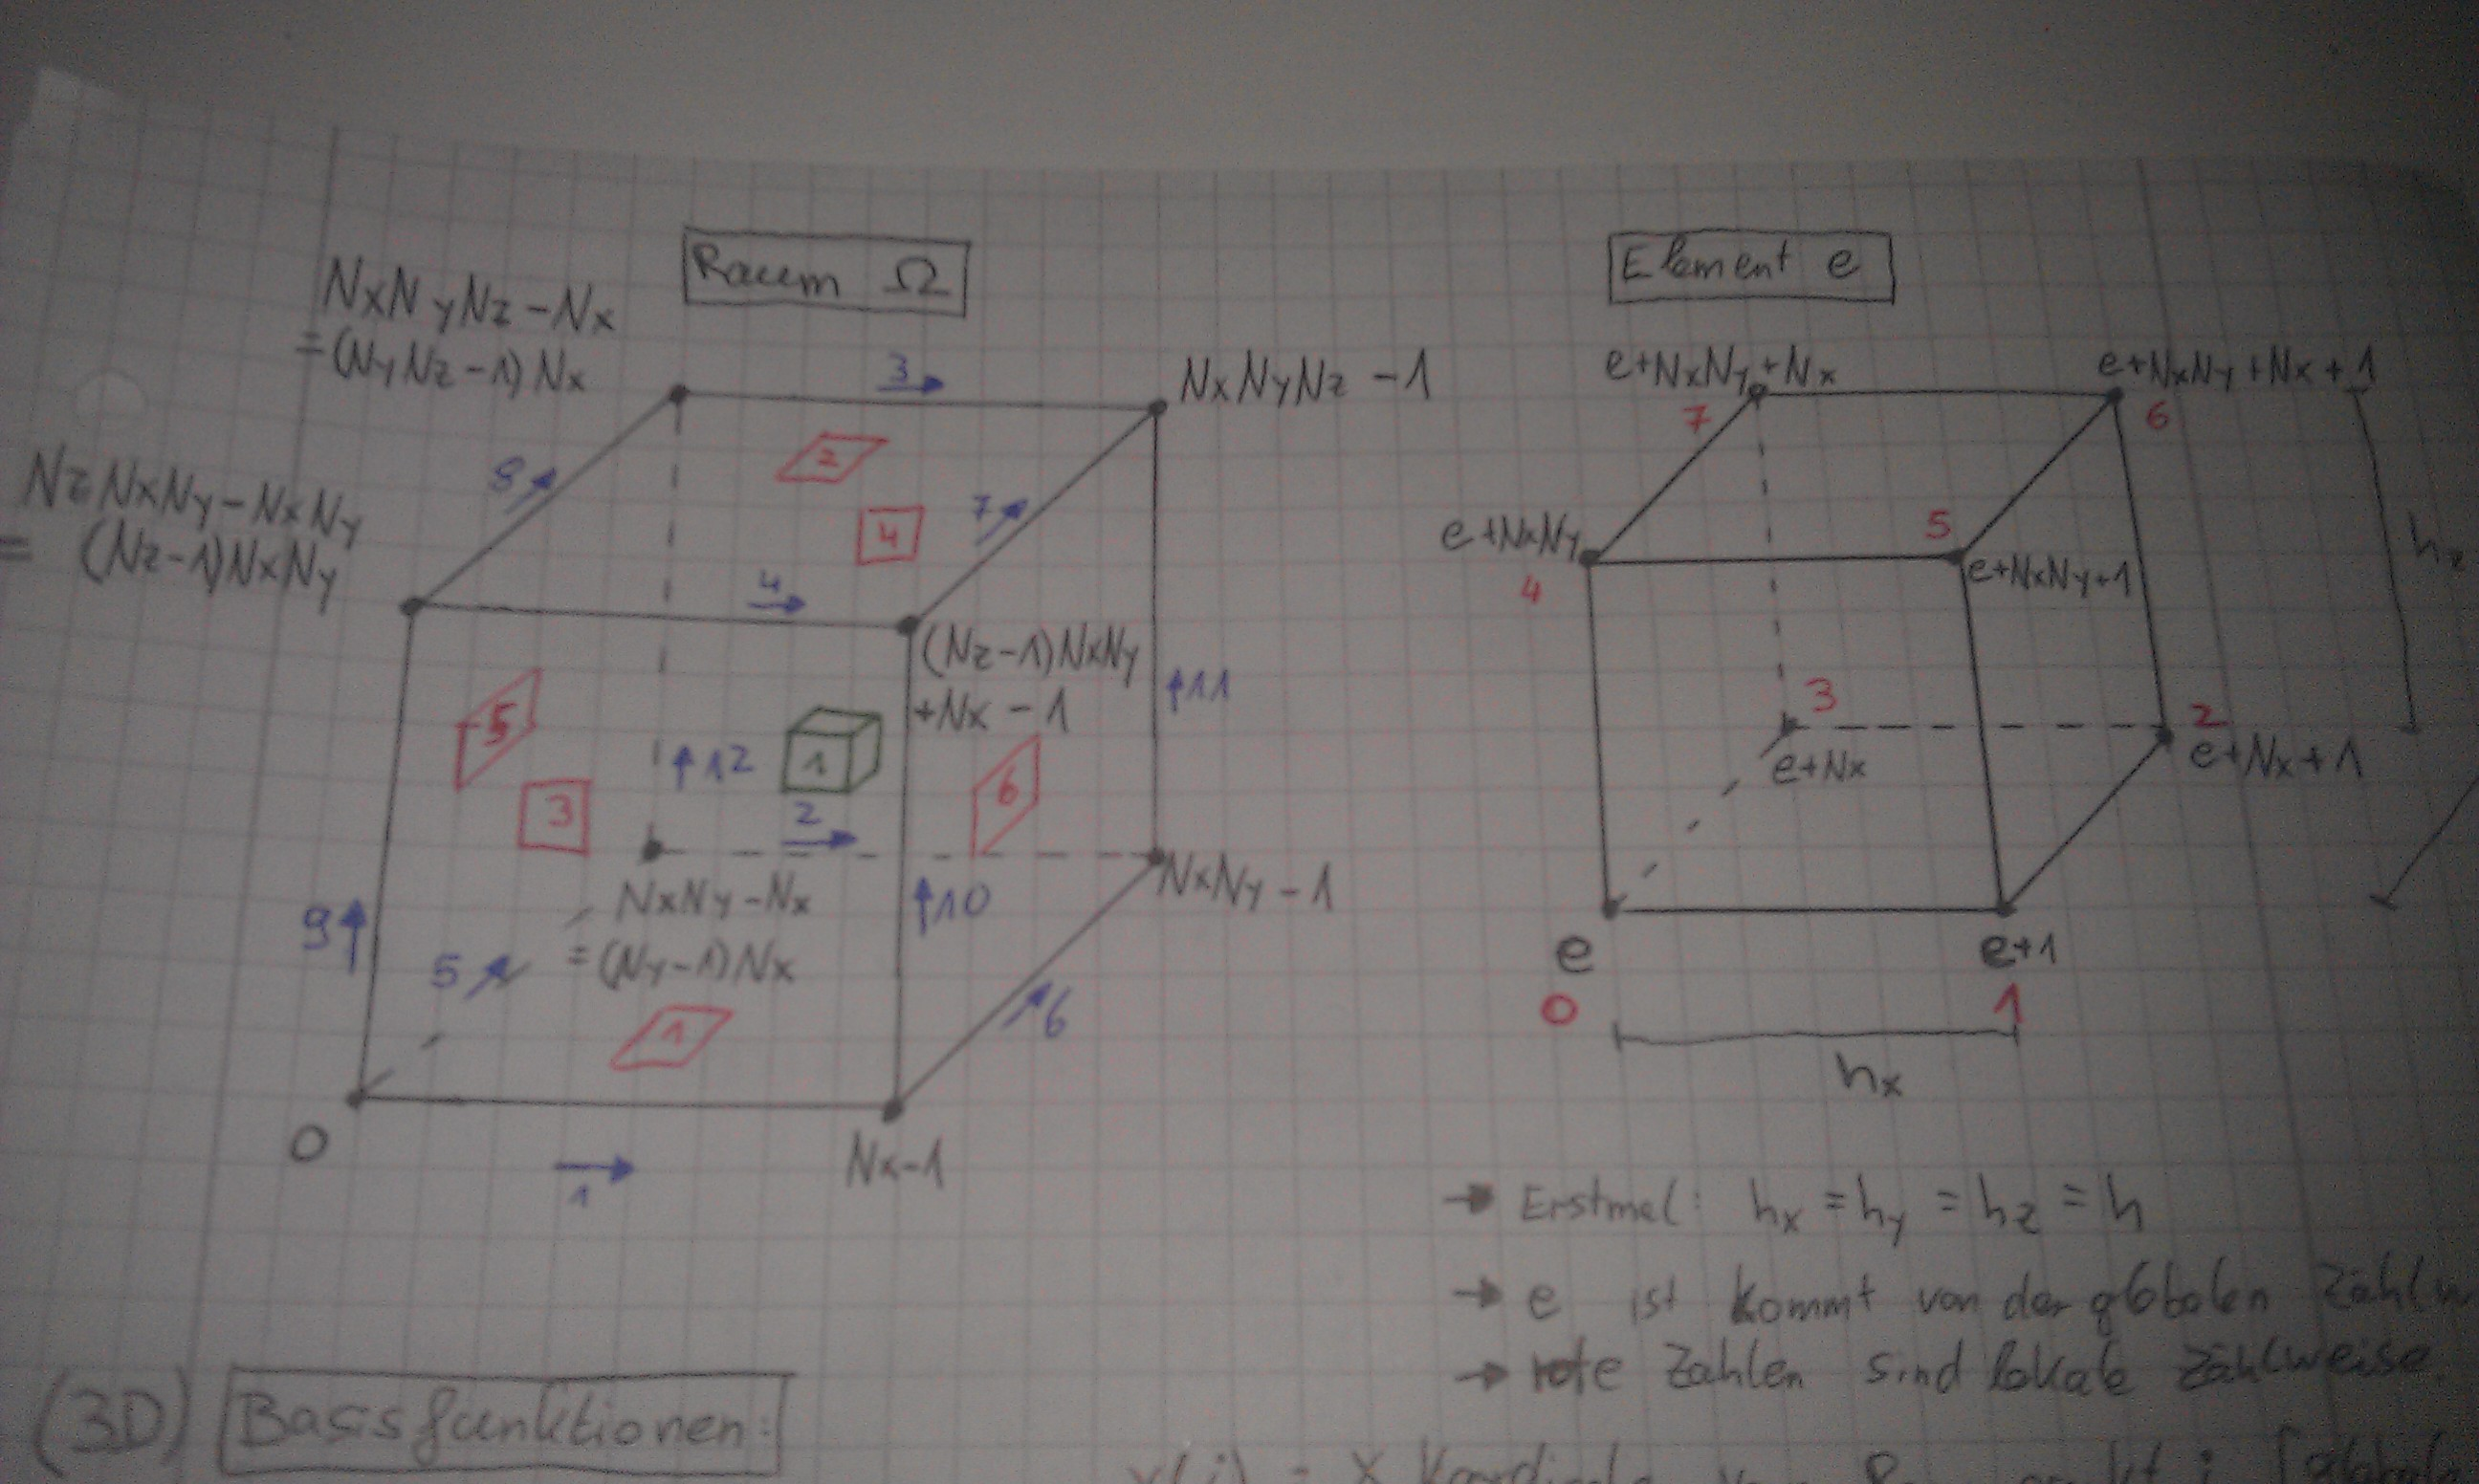
\includegraphics[scale=0.15]{./Bilder/draft}
		
		\caption{Raum $\Omega$ und Element mit Nummerierung}\label{draft}
	\end{center}
\end{figure}

Als Gebiet wird ein Quader $\Omega \subset \mathbb{R}^{3}$ betrachtet, der mit einem äquidistanten Gitter so überdeckt wird, dass eine Triangulierung $T_h$ aus Würfeln mit der Kantenlänge $h$ entsteht. \\
Die Punkte des Gitters werden nun global durchnummeriert, angefangen mit dem linken, unteren, vorderen Punkt des Quaders, er erhält den Index 0. Man zählt zunächst in x-Richtung (Nx = Anzahl Gitterpunkte in x-Richtung, ebenso Ny und Nz) durch, dann in y-Richtung und dann in z-Richtung. Insgesamt gibt es also $Nx \cdot Ny \cdot Nz$ Gitterpunkte. Der aktuell betrachtete, globale Index erhält die Variable \glqq Zeile\grqq. Diesem Index wird eindeutig ein Element zugewiesen, indem der Punkt des Gitters mit diesem Index der linken unteren, vorderen Ecke des Elementes entspricht. Ebenso muss eine lokale Nummerierung eines einzelnen Elementes vorgenommen werden, diese entnehme man Abbildung \ref{draft}.\\

Bevor man nun die Matrix $A$ aufstellen kann, muss man sich mit der Theorie der FEM für das vorliegende Problem beschäftigen. 
Aus der Poisson-Gleichung erhält man die schwache Formulierung 
\begin{equation}
a(u, \varphi)=l( \varphi) \text{ } \forall \varphi \in V:=H^1_0 
\end{equation} \label{Gl1}


mit der Bilinearform $a(u, \varphi)=\int_\Omega \! \nabla u \nabla \varphi \, \mathrm{d}x $ und der Linearform $l( \varphi)= \int_\Omega \! f \varphi \, \mathrm{d}x $. Anschließend wird die schwache Form mit einem endlich-dimensionalen Raum $V_h \subset V$ diskretisiert. Mit einer Basis $(\varphi_i)_{i=1,...,N}$ von $V_h$ und Ausnutzen der Bilinearität ist \eqref{Gl1} im diskreten Fall äquivalent zu 
\begin{equation}
\sum_{i=1}^N u_i a(\varphi_i, \varphi_j)=l(\varphi_j) \text{ } , \text{ } j = 1,...,N,
\end{equation}
wobei dann $A u = b$ mit $a_{ji}=a(\varphi_i, \varphi_j)$ und $b_j=l(\varphi_j)$. \\

Es bleiben die Einträge der Systemmatrix und der rechten Seite zu berechnen. 
Die Basis  wird in 3D so gewählt, dass sie auf einem Element trilinear ist. Zur Einbindung von Randbedingungen sind außerdem Basisfunktionen in 2D aufzustellen, diese sind bilinear auf einem Quadrat. Die Basen werden durch den Lagrangeschen Basispolynomansatz gebildet. Bei der FEM koppelt man die Basis $\varphi_i$ von einem Punkt $i$ mit den Basisfunktionen aller anderen Punkte des Netzes. Aufgrund der Wahl der Basis reicht es jedoch, die direkt umliegenden Punkte zu betrachten, da für alle anderen Punkte $j$ gilt: $supp(\varphi_i) \cap supp(\varphi_j) = \emptyset$. Allerdings ergeben sich für Punkte, die auf dem Rand $\partial \Omega$ liegen, Sonderfälle, weil es dort im Gegensatz zu den inneren Punkten weniger umliegende Punkte gibt. Man muss dann unterscheiden, ob sich ein Punkt in einer Ecke, auf einer Kante oder auf einer Seitenfläche des Quaders $\Omega$ befindet. Dies erklärt die unterschiedlichen Schleifen in der Implementierung der FEM. \\
Die Integrale, die zum Aufstellen des LGS bestimmt werden müssen, rechnet man mit einer Quadraturformel aus, die in diesem Fall einer 27-Punkt-Gauss-Formel in 3D und einer 9-Punkt-Gauss-Formel in 2D entspricht (auch hier: zweidimensionale Integrale müssen beispielsweise bei Berücksichtigung der Randbedingungen berechnet werden). \\
Die Berechnung der Gauss-Punkte und die Auswertung der Funktionen werden auf einem Referenzelement durchgeführt. In 3D entspricht dieses $RE3=[0,h]^3$ und in 2D $RE2=[0,h]^2$. Dabei sind die aus diesem Ansatz resultierenden Transformationen vom Referenzelement auf die Elemente der Triangulierung reine Translationen. Die Referenz\-elemente haben den Nutzen, dass die Gauss-Punkte lediglich ein einziges Mal evaluiert bzw. die Funktionen nur ein Mal ausgewertet werden müssen.   \\

Insgesamt hat die Verwendung der FEM den Vorteil, dass die Assemblierung der Matrix $A$ leicht parallelisierbar ist, indem man die einzelnen Raumpunkte durchläuft, da sich durch einen Raumpunkt eine gesamte Zeile des LGS berechnen lässt. Desweiteren lassen sich, falls bei einem Problem vorhanden, Neumann-Randbedingungen wesentlich einfacher einbinden als z.B. bei den Finiten Differenzen. 


\subsection{Löser}
Das als Löser verwendete Verfahren des Projektes ist das sogenannte BiCGStab-\newline Verfahren (engl: „biconjugate gradient stabilized method“), welches zur Klasse der Krylov-Unterraum-Verfahren zählt. Diese iterative Methode wurde von H.A. van der Horst als Löser für nicht-symmetrische lineare Gleichungssysteme entwickelt und benötigt keine zusätzlichen Anforderungen an die Systemmatrix A wie zum Beispiel das CG-Verfahren. Sein Name ist davon abgeleitet, dass die im nicht-vorkonditionierten Algorithmus verwendeten Residuen biorthogonal sind, also $(r_i,\hat{r}_j)=\,0$ $\forall i\neq j$, und die Suchrichtungen bikonjugiert sind bezüglich der Systemmatrix $A$, also $(Ap_i,\hat{p}_j)=\,0$ $ \forall i \neq j$.  Man verwendet dieses Verfahren, da das konkurrierende GMRES-Verfahren weniger speichereffizient arbeitet und das BiCGStab-Verfahren leichter zu implementieren ist.  Au\ss{}erdem kann es mit beliebigem Vorkonditionierer und ohne Vorkonditionierer implementiert werden. Der Nachteil des angewendeten Verfahrens ist, dass die Konvergenz nicht allgemein bewiesen ist.  \\



\begin{enumerate}
	\setlength{\itemsep}{-6pt}
\hrule\hrule
	
	
	\item $r_0$=$b$-$A$$x_0$
	\item $\hat{r}_0$=$r_0$
	\item $\rho_0$=$\alpha$=$\omega_0$=1
	\item $v_0$=$p_0$=0
	\item for $i$=1,2,\dots
	\par
	\begingroup
	\leftskip=0,6cm 
	\noindent 
	\item$\rho_i=$\,($\hat{r_0}$,$r_{i-1}$)
	\item$\beta=$\,($\rho_i$/$\rho_{i-1}$)($\alpha$/$\omega{i-1}$)
	\item$p_i=$\,$r_{i-1}$+$\beta$($p_{i-1}-\omega_{i-1}v_{i-1}$)	
	\item$y=$\,$K^{-1}p_i$
	\item$v_i=$\,$Ay$
	\item$\alpha=$\,$\rho_i/(\hat{r_0},v_i)$
	\item$s=$\,$r_{i-1}-\alpha$$v_i$
	\item Wenn $||s|| < TOL$, setze $x_i=$\,$x_{i-1}+\alpha$$p_i$ und beende 
	\item$z=$\,$K^{-1}s$
	\item$t=$\,$Az$
	\item$\omega_i=$\,$(K^{-1}_1$$t,K^{-1}_1$$s)/(K^{-1}_1$$t,K^{-1}_1$$t)$ 
	\item$x_i=$\,$x_{i-1}+\alpha$$y+\omega_i$$z$
	\item$r_i=$\,$s-\omega_i$$t$\\
	
	\hrule\hrule
	\par
	\endgroup 
	
\end{enumerate}



Der von rechts vorkonditionierte BiCGSTAB-Algorithmus startet ausgehend von einem Anfangsvektor $x_0$, welcher immer als Nullvektor implementiert wurde. Des Weiteren wurde die Toleranz mit $TOL= 10^{-9}$ festgelegt. Der Vorkonditionierer hat dabei die allgemeine Form: 
$K = K_1 K_2 \approx A $

\subsection{Matrixformat}

Sowohl mit der Finite-Elemente-Methode, als auch mit Finiten Differenzen als Diskretisierungsansatz, entstehen bei der Übersetzung Partieller Differentialgleichungen in Lineare Gleichungssysteme Systemmatrizen $A \in \mathbb{R}^{M \times M},~M \in \mathbb{N}$  mit hochgradig dünnbesetzer Struktur. Auf $M^2$ Gesamteinträge kommen, bei Verwendung der Finiten-Elemente-Methode, etwa $27M$ Nichtnull-Einträge, bei Finiten Differenzen $7M$. Diese sind bei durchgehender globaler Nummerierung und konstanten Gitterweiten $N_x,N_y,N_z$ auf einem Band der Breite $\sim 2 N_x (N_y+1)$ bzw. $\sim 2 N_xN_y$ verteilt. Abbildung xy zeigt schematisch die Besetzungsstrukturen der Matrizen.\\

\textit{Abbildung zur Besetzungsstruktur folgt}\\

Um nun auch große Probleme lösen zu können, ist es wichtig die Sparse-Eigenschaft der Matrizen beim Speichern zu respektieren. Das ELLPACK Speicherformat erfüllt eben dies und erlaubt die im BiCGStab auftretenden Sparsematrix-Vektor Operationen auf mehreren Knoten verteilt zu berechnen.\\
In der praktischen Umsetzung werden dazu mehrere Zeilen der Systemmatrix einer Node zugeordnet und dort im ELLPACK Format gespeichert. Dabei werden alle Nulleinträge aus der Matrix entfernt, sodass die übrigen Einträge zeilenweise linksbündig anliegen. Die längste Zeile bestimmt die Breite der Matrix - eventuelle Lücken in anderen Zeilen werden mit Nullen aufgefüllt. Die Spaltenindizes zu jedem Eintrag werden in einer zweiten Matrix gespeichert. Die enstandenen Matrizen werden dann von oben nach unten orientiert gespeichert. Sparsematrix-Vektor Multiplikation $y=Ax$ können nun elementweise als $y_i = \sum \limits_{nz=0}^{nz_i} A_{i,nz} x_{j_{nz}}$ berechnet werden, wobei $nz_i$ die Anzahl der Nichtnull Einträge in Zeile $i$ ist. Da dies vollkommen unabhängig für jede Zeile - und damit für jede Node - geschieht, gibt es eine Antiproportionalität zwischen Rechenzeit und Anzahl der Nodes. Zu beachten ist aber der erhöhte kommunikative Aufwand zwischen den Nodes, da der Ergebnisvektor y ausschließlich verteilt gespeichert ist.\\

\textit{Abbildung zur ELLPACK-Funktionsweise folgt}\\
